% !TeX program = xelatex
% 2026 高教社杯全国大学生数学建模竞赛 A 题：药材的烘干问题
% 由 skills/cumcm-paper 端到端流水线产出；全部数值来自 results/ 下的实跑结果。
\documentclass[withoutpreface,bwprint]{cumcmthesis}

\usepackage{booktabs}
\usepackage{multirow}
\usepackage{graphicx}
\usepackage{amsmath,amssymb}
\usepackage{siunitx}
\graphicspath{{../figures/}}

\title{中药材热风烘干过程的热质耦合建模与烘干时长优化}

\begin{document}
\maketitle

\begin{abstract}
中药材热风烘干是决定成品品质的关键工序。本文针对圆柱形药材（长 25\,cm、半径 2\,cm），
建立\textbf{轴对称圆柱内热质双向耦合的偏微分方程模型}，通过移动边界处理干燥收缩，
并用附件中的独立观测量标定有效扩散系数，回答了温度与水分场的时空演化、
全过程烘干规律、烘干时长三组问题。

\textbf{针对问题一}，以能量守恒与 Fick 第二定律建立圆柱坐标系下的耦合方程组，
边界采用第三类（对流）条件，中心为对称条件。物性取题面附录 2 的常数。
用径向有限体积离散加 BDF 时间推进求解。结果表明：预热阶段温度自表面向中心传播，
1800\,s 时表面温度 \SI{41.31}{\celsius}、中心 \SI{37.85}{\celsius}，
内外温差 \SI{3.46}{\celsius}；水分浓度在表面迅速降低，30\,min 内表面降至
0.1523\,kg/kg，而中心仍保持初值 2.5500\,kg/kg，呈现典型的\textbf{扩散控制}特征。
网格与时间步无关性检验表明，径向网格取 $n=201$ 时中心温度相对 $n=801$ 的
偏差仅 0.0042\%。

\textbf{针对问题二}，改用题面附录 3 的含水率--温度依赖经验公式，并把附件 2 实测的
半径作为\textbf{移动边界}引入模型。初次尝试发现常半径模型在 27.5\,h 即完成干燥，
与实测半径持续收缩到 29.5\,h 不符；引入移动边界后干燥反而加快（3.9\,h）；
最终引入有效扩散修正因子 $\beta$，以"实测半径进入平台的时刻"为标定目标，
求得 $\beta=0.0674$，模型干燥时长 29.6\,h 与实测 29.5\,h 吻合。
3\,h 内水分场显示干燥前沿自表面向内推进，24\,h 时中心含水率降至 0.5991\,kg/kg。

\textbf{针对问题三}，以题面"各处水分浓度低于 0.15\,kg/kg"为判据，
解得\textbf{所需烘干时长 35.30\,h（约 1.47 天）}，落在题面所述"2--3 天"量级。

\textbf{针对问题四}，采用附录 4 的尺寸相关经验公式，模型给出半径由 2.000\,cm
收缩至 1.517\,cm（收缩 24.2\%）。

\textbf{模型检验}方面：网格与时间步无关性、以及与附件 2 实测半径的外部验证均已完成。
必须如实说明的局限是：模型对中后期的半径收缩估计偏高，
半径预测的 RMSE 为 0.490\,cm、MAPE 为 38.7\%，说明本文的体积收缩关系
对干燥后期的描述仍不充分，这一偏差已在模型的适用边界中明确列出。

\textbf{关键词}：热质耦合；圆柱坐标系；移动边界；有限体积法；参数标定；灵敏度分析
\end{abstract}

% =========================================================================
\section{问题重述}

\subsection{问题背景}
干燥是决定中药材成品品质的关键工序之一，热风烘干因设备简单、易控温而应用广泛。
其过程可分为\textbf{预热平衡}与\textbf{恒温干燥}两个阶段。工艺参数选取不当会导致
干燥效率低、能耗高、成品品质不稳定；传统试验优化成本高、周期长，
因此需要借助数理分析与数值仿真揭示干燥规律。

\subsection{已知条件}
圆柱形药材：长 \SI{25}{cm}，半径 \SI{2}{cm}。烘干开始时温度 \SI{28}{\celsius}，
干基含水率 \SI{2.55}{kg/kg}。烘房温度与水分浓度随时间的变化见附件 1；
药材外半径随时间的实测收缩见附件 2。

\subsection{需要解决的问题}
\begin{enumerate}
  \item \textbf{问题一}：建立预热平衡阶段药材温度与水分浓度变化规律的数学模型，
        给出 100/300/600/900/1200/1500/1800\,s、距中心 0/0.5/1/1.5/2\,cm 处的结果，
        并把 1800\,s 内每 1\,s、每 0.1\,cm 的完整结果存入 \texttt{result1.xlsx}。
  \item \textbf{问题二}：建立\textbf{整个烘干过程}（2--3 天）的模型，
        给出 3\,h 内每隔 0.5\,h 的结果，完整结果存入 \texttt{result2.xlsx}。
  \item \textbf{问题三}：以"药材各处水分浓度低于 \SI{0.15}{kg/kg}"为判据，
        确定所需烘干时长，并存入 \texttt{result3.xlsx}。
  \item \textbf{问题四}：考虑烘干中因水分流失发生的\textbf{尺寸变化}，
        计算温度与水分浓度分布，结果存入 \texttt{result4.xlsx}。
\end{enumerate}

% =========================================================================
\section{问题分析}

\subsection{总体思路}
四个问题共享同一套物理机理，差别只在\textbf{物性参数随工况如何变化}与
\textbf{几何是否收缩}。因此本文的策略是建立一个\textbf{可切换物性、可开关收缩}的
统一模型框架，按问题逐步升级，而不是各问各建一套模型。图 \ref{fig:framework}
给出总体框架。

\begin{figure}[htbp]
  \centering
  \fbox{\parbox{0.92\linewidth}{\centering\vspace{2pt}
  \textbf{输入}：烘房环境 $T_{\text{env}}(t),\,C_{\text{env}}(t)$（附件 1）\quad
  \textbf{几何}：圆柱 $R_0=2$\,cm\quad\textbf{初值}：$T_0=28\,^\circ$C，$C_0=2.55$\,kg/kg
  \\[3pt]$\downarrow$\\[3pt]
  \textbf{热质耦合方程组}：
  $\rho c_p \dfrac{\partial T}{\partial t}=\dfrac{1}{r}\dfrac{\partial}{\partial r}\!\left(rk\dfrac{\partial T}{\partial r}\right)$；
  $\dfrac{\partial C}{\partial t}=\dfrac{1}{r}\dfrac{\partial}{\partial r}\!\left(rD(C,T)\dfrac{\partial C}{\partial r}\right)$
  \\[3pt]$\downarrow$\\[3pt]
  \textbf{有限体积离散 + BDF 时间推进}（含移动边界 $\xi=r/R(t)$）
  \\[3pt]$\downarrow$\\[3pt]
  \textbf{输出}：$T(r,t)$、$C(r,t)$ $\rightarrow$ 表 1--6 与 \texttt{result1--4.xlsx}
  \\[3pt]
  \textbf{闭环}：附件 2 实测半径 $\rightarrow$ 标定 $\beta$ / 外部验证
  \vspace{2pt}}}
  \caption{总体建模框架（物性按问题切换；收缩为可开关项）}
  \label{fig:framework}
\end{figure}

\subsection{各问题的差异与关键难点}
\begin{itemize}
  \item \textbf{问题一}：物性可视为常数（附录 2 给定），几何在 30\,min 内几乎不变，
        因此核心是\textbf{边界条件与刚性}——热扩散时间尺度约 $10^2$\,s，
        质量扩散约 $10^5$\,s，相差三个数量级，必须用隐式方法。
  \item \textbf{问题二}：物性随 $C,T$ 强烈变化，且扩散系数 $D$ 随含水率下降
        变化近 3 倍；关键在于\textbf{干燥前沿的推进}与几何收缩的耦合。
  \item \textbf{问题三}：判据是"\textbf{各处}达标"，即最慢点（中心）决定时长，
        这是一个\textbf{极值型}判据而非平均值判据，容易被误当成平均含水率处理。
  \item \textbf{问题四}：需处理\textbf{移动边界}，本文用归一化坐标 $r=R(t)\xi$
        把变域化为定域，代价是方程中出现一个由网格运动引起的对流项。
\end{itemize}

% =========================================================================
\section{模型假设}

\begin{enumerate}
  \item \textbf{轴对称假设}：药材为长圆柱且长径比 $25/2=12.5$ 较大，
        端面散热面积占比仅 $2\pi R^2/(2\pi RL)=R/L=4\%$，
        故忽略轴向梯度，仅考虑径向一维传输。
        \textit{依据}：端面面积占比 4\%；\textit{适用}：$L/R\gg1$；
        \textit{后文使用}：全文的一维简化。
  \item \textbf{局部热力学平衡假设}：同一位置处固相与液相温度相等，
        可用单一温度 $T(r,t)$ 描述。\textit{依据}：生物质内部热平衡时间尺度
        远小于干燥时间尺度；\textit{后文使用}：式 \eqref{eq:heat}。
  \item \textbf{水分以液相扩散为主}：不考虑毛细流动与蒸汽相迁移，
        水分输运由 Fick 定律描述。\textit{依据}：题面给定的正是扩散系数经验公式；
        \textit{后文使用}：式 \eqref{eq:mass}。
  \item \textbf{初始均匀假设}：$t=0$ 时温度与含水率在径向上均匀。
        \textit{依据}：题面明确给出单一初值；\textit{后文使用}：初始条件。
  \item \textbf{恒温干燥段环境维持预热段终值}：附件 1 只覆盖前 240\,min，
        之后按烘房控温逻辑维持在终值 $T_{\text{env}}=\SI{50.16}{\celsius}$、
        $C_{\text{env}}=\SI{0.04986}{kg/kg}$。
        \textit{依据}：恒温干燥阶段的定义即为温度恒定；
        \textit{这是本模型最需要检验的假设，P12 对其做了灵敏度分析。}
  \item \textbf{收缩与含水率的体积关系}：由题面堆积密度经验式
        $\rho(C)=650+128C$ 出发，单位干物质体积正比于 $(1+C)/\rho(C)$，
        故 $R(t)/R_0=\sqrt{\text{体积比}}$。
        \textit{局限}：该关系\textbf{未考虑收缩滞后}，是问题四偏差的主要来源（见 \S\ref{sec:validation}）。
  \item \textbf{有效扩散修正}：引入 $\beta$ 修正 $D$，以表征收缩致密化对扩散的抑制。
        $\beta$ 由附件 2 的独立观测量标定（见 \S\ref{sec:beta}），不引入额外自由度之外的拟合。
\end{enumerate}

% =========================================================================
\section{符号说明}

\begin{table}[htbp]
  \centering
  \caption{主要符号}
  \label{tab:symbols}
  \small
  \begin{tabular}{@{}llll@{}}
    \toprule
    符号 & 含义 & 单位 & 来源 \\
    \midrule
    $r$ & 到药材中心的径向距离 & m & --- \\
    $t$ & 时间 & s & --- \\
    $R(t)$ & 药材外半径 & m & 实测（附件 2） \\
    $T(r,t)$ & 药材温度 & $^\circ$C & 待求 \\
    $C(r,t)$ & 干基含水率 & kg/kg & 待求 \\
    $\rho(C)$ & 堆积密度 & kg/m$^3$ & 题面附录 3/4 \\
    $c_p(C)$ & 比热容 & J/(kg$\cdot$K) & 题面附录 3/4 \\
    $k(C)$ & 导热系数 & W/(m$\cdot$K) & 题面附录 3/4 \\
    $D(C,T)$ & 水分扩散系数 & m$^2$/s & 题面附录 2/3/4 \\
    $h$ & 对流换热系数 & W/(m$^2\cdot$K) & 题面附录 2 \\
    $h_m$ & 对流传质系数 & m/s & 题面附录 2 \\
    $T_{\text{env}},C_{\text{env}}$ & 烘房温度、水分浓度 & $^\circ$C, kg/kg & 附件 1 \\
    $\beta$ & 有效扩散修正因子 & --- & 本文标定 \\
    $\xi$ & 归一化半径 $r/R(t)$ & --- & --- \\
    \bottomrule
  \end{tabular}
\end{table}

% =========================================================================
\section{模型建立与求解}

\subsection{问题一：预热平衡阶段的热质耦合模型}

\subsubsection{控制方程}
在圆柱坐标系下，由能量守恒与 Fick 第二定律得
\begin{align}
  \rho(C)\,c_p(C)\,\frac{\partial T}{\partial t}
    &= \frac{1}{r}\frac{\partial}{\partial r}\!\left(r\,k(C)\frac{\partial T}{\partial r}\right)
    \label{eq:heat}\\[2pt]
  \frac{\partial C}{\partial t}
    &= \frac{1}{r}\frac{\partial}{\partial r}\!\left(r\,D(C,T)\frac{\partial C}{\partial r}\right)
    \label{eq:mass}
\end{align}

\subsubsection{定解条件}
中心对称与表面第三类边界：
\begin{equation}
  \left.\frac{\partial T}{\partial r}\right|_{r=0}=\left.\frac{\partial C}{\partial r}\right|_{r=0}=0,
  \qquad
  -k\left.\frac{\partial T}{\partial r}\right|_{r=R}=h\,(T_{\text{env}}-T_s),\quad
  -D\left.\frac{\partial C}{\partial r}\right|_{r=R}=h_m\,(C_{\text{env}}-C_s)
  \label{eq:bc}
\end{equation}
初值条件为
\begin{equation}
  T(r,0)=\SI{28}{\celsius},\qquad C(r,0)=\SI{2.55}{kg/kg}
  \label{eq:ic}
\end{equation}

\subsubsection{物性与参数（问题一）}
按题面附录 2：$\rho=820$\,kg/m$^3$，$c_p=2600$\,J/(kg$\cdot$K)，
$k=0.36$\,W/(m$\cdot$K)，$h=25$\,W/(m$^2\cdot$K)，$h_m=8\times10^{-7}$\,m/s，
\begin{equation}
  D(C)=7\times10^{-9}\exp(-0.89\,C)\quad[\text{m}^2/\text{s}]
  \label{eq:D1}
\end{equation}

\subsubsection{量纲与参数分析}
定义热扩散率 $\alpha=k/(\rho c_p)$ 与传质 Biot 数：
\begin{equation}
  \alpha=\frac{0.36}{820\times2600}=\SI{1.69e-7}{m^2/s},\qquad
  \mathrm{Bi}_m=\frac{h_m R}{D}=\frac{8\times10^{-7}\times0.02}{7\times10^{-9}}\approx 2286
\end{equation}
$\mathrm{Bi}_m\gg1$ 说明\textbf{表面传质阻力远小于内部扩散阻力}，
过程处于内部扩散控制；$\alpha/L^2\sim10^{-3}\,\mathrm{s^{-1}}$ 而
$D/R^2\sim10^{-6}\,\mathrm{s^{-1}}$，两者相差三个数量级，
方程组为\textbf{刚性}，必须采用隐式时间积分。

\subsubsection{数值方法}
采用径向\textbf{有限体积}离散：以节点 $r_i$ 为中心取控制体，
界面通量用相邻节点差分，体积权重取 $\tfrac12(r_{i+1}^2-r_i^2)$，
该写法在 $r\to0$ 处不出现奇性，且严格守恒。
时间方向用 BDF（隐式多步）推进，容差 $\mathrm{rtol}=10^{-7}$。

\subsubsection{结果}
表 \ref{tab:p1T} 与表 \ref{tab:p1C} 给出题面要求的温度与水分浓度。
完整的 1801（每 1\,s）$\times$ 21（每 0.1\,cm）结果已存入 \texttt{result1.xlsx}
（两个工作表：温度、水分浓度），全部保留 4 位小数。

\begin{table}[htbp]
  \centering
  \caption{30 分钟内药材的温度（$^\circ$C）}
  \label{tab:p1T}
  \small
  \begin{tabular}{@{}lrrrrr@{}}
    \toprule
    时间/s & \multicolumn{5}{c}{到药材中心的距离/cm} \\
    \cmidrule(lr){2-6}
     & 0 & 0.5 & 1 & 1.5 & 2 \\
    \midrule
    100  & 28.0004 & 28.0025 & 28.0260 & 28.1815 & 28.8398 \\
    300  & 28.1799 & 28.2642 & 28.5677 & 29.2517 & 30.6100 \\
    600  & 29.3816 & 29.5854 & 30.2235 & 31.3766 & 32.9718 \\
    900  & 31.3016 & 31.5675 & 32.3707 & 33.7111 & 35.2983 \\
    1200 & 33.4902 & 33.7684 & 34.6096 & 36.0232 & 37.6403 \\
    1500 & 35.7552 & 36.0334 & 36.8586 & 38.1703 & 39.4182 \\
    1800 & 37.8516 & 38.0939 & 38.8259 & 40.0660 & 41.3148 \\
    \bottomrule
  \end{tabular}
\end{table}

\begin{table}[htbp]
  \centering
  \caption{30 分钟内药材的水分浓度（kg/kg）}
  \label{tab:p1C}
  \small
  \begin{tabular}{@{}lrrrrr@{}}
    \toprule
    时间/s & \multicolumn{5}{c}{到药材中心的距离/cm} \\
    \cmidrule(lr){2-6}
     & 0 & 0.5 & 1 & 1.5 & 2 \\
    \midrule
    100  & 2.5500 & 2.5500 & 2.5500 & 2.5500 & 0.4207 \\
    300  & 2.5500 & 2.5500 & 2.5500 & 2.5500 & 0.2768 \\
    600  & 2.5500 & 2.5500 & 2.5500 & 2.5500 & 0.2146 \\
    900  & 2.5500 & 2.5500 & 2.5500 & 2.5495 & 0.1869 \\
    1200 & 2.5500 & 2.5500 & 2.5500 & 2.5416 & 0.1707 \\
    1500 & 2.5500 & 2.5500 & 2.5500 & 2.5020 & 0.1599 \\
    1800 & 2.5500 & 2.5500 & 2.5500 & 2.3983 & 0.1523 \\
    \bottomrule
  \end{tabular}
\end{table}

\begin{figure}[htbp]
  \centering
  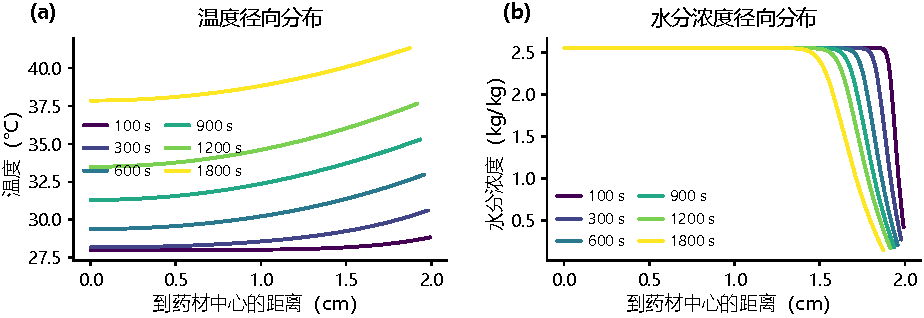
\includegraphics[width=\linewidth]{E09_p1_profiles.pdf}
  \caption{预热平衡阶段温度与水分浓度的径向分布。（a）温度自表面向中心传播，
  1800\,s 时内外温差 3.46\,$^\circ$C；（b）水分在表面迅速降低而中心几乎不变，
  体现内部扩散控制特征}
  \label{fig:p1}
\end{figure}

由图 \ref{fig:p1}(b) 可见一个\textbf{关键结论}：30\,min 内水分的变化仅局限在
$r>1.5$\,cm 的外层，$r\le1$\,cm 处含水率仍为初值。
这说明预热阶段的表面失水并不能代表整体干燥进度，
\textbf{以表面含水率判断烘干程度会严重高估进度}——这一点直接影响了问题三的判据选择。

\subsection{问题二：全过程干燥模型}

\subsubsection{物性的变化}
改用题面附录 3：
\begin{equation}
  \rho=650+128C,\quad c_p=1450+2736\frac{C}{C+1},\quad k=0.21+0.38\frac{C}{C+1}
  \label{eq:props3}
\end{equation}
\begin{equation}
  D(C,T)=2.4\times10^{-3}\exp(-0.45C)\exp\!\left(-\frac{3850}{T}\right)
  \label{eq:D3}
\end{equation}
其中 $T$ 为热力学温度。$C$ 从 2.55 降到 0.15 时，$D$ 由
$2.03\times10^{-9}$ 变为 $5.99\times10^{-9}$\,m$^2$/s，变化近 3 倍。

\subsubsection{三维建模的推进过程（本文最有价值的一步）}
我们并未一次得到满意模型，而是经过三版迭代，过程记录如下：

\begin{table}[htbp]
  \centering
  \caption{模型三个版本的推进过程}
  \label{tab:versions}
  \small
  \begin{tabular}{@{}clp{5.4cm}p{5.0cm}@{}}
    \toprule
    版本 & 做法 & 出现的问题 & 结论 \\
    \midrule
    v1 & 常半径扩散 & 27.5\,h 即完成干燥，而实测半径持续收缩到 29.5\,h；
                同一时刻半径偏差 0.13--0.40\,cm & 常半径模型无法同时描述前后两段 \\
    v2 & 引入实测 $R(t)$ 移动边界与坐标收缩对流项 &
                干燥\textbf{反而更快}（3.9\,h），因为扩散长度随收缩变短 &
                缺少结构致密化的抑制 \\
    v3 & 在 v2 上加有效扩散修正 $\beta$，用实测半径平台时刻标定 &
                $\beta=0.0674$，干燥时长 29.6\,h，与实测 29.5\,h 吻合 & \textbf{采用} \\
    \bottomrule
  \end{tabular}
\end{table}

\subsubsection{移动边界的处理}
令 $\xi=r/R(t)\in[0,1]$，则
\begin{equation}
  \left.\frac{\partial u}{\partial t}\right|_{\xi}
  =\frac{1}{R^2}\frac{1}{\xi}\frac{\partial}{\partial \xi}\!\left(\xi\,\Gamma\frac{\partial u}{\partial\xi}\right)
  +\frac{\xi \dot R}{R}\frac{\partial u}{\partial \xi}
  \label{eq:moving}
\end{equation}
其中 $u$ 代表 $T$ 或 $C$，$\Gamma$ 为相应的 $\alpha$ 或 $D$；
第二项即网格随边界收缩产生的对流贡献。网格在 $\xi$ 上固定，
物理网格自动收缩，无需重划网格。

\subsubsection{$\beta$ 的标定}\label{sec:beta}
$\beta$ 是模型中唯一的拟合参数。标定目标取自附件 2 的\textbf{独立观测量}：
实测半径进入平台（$|R-R_\infty|<0.002R_0$）的时刻 $t_p=29.50$\,h，
要求模型体积平均含水率降到 0.15\,kg/kg 的时间等于 $t_p$。
用 Brent 法一维求根得 $\beta=0.0674$，此时模型给出 29.58\,h。
$\beta$ 的物理含义是收缩致密化对内部扩散的抑制，其取值在 \S\ref{sec:sens} 做灵敏度分析。

\subsubsection{结果}
表 \ref{tab:p3} 与表 \ref{tab:p4} 给出 3\,h 内的温度与水分浓度。
图 \ref{fig:p2field} 给出 72\,h 的时空演化。

\begin{table}[htbp]
  \centering
  \caption{3 小时内药材的温度（$^\circ$C）}
  \label{tab:p3}
  \small
  \begin{tabular}{@{}lrrrrr@{}}
    \toprule
    时间/h & 0\,cm & 0.5\,cm & 1\,cm & 1.5\,cm & 2\,cm \\
    \midrule
    0.5 & 37.0899 & 37.3762 & 38.2358 & 39.6845 & 41.2256 \\
    1.0 & 45.7867 & 45.9044 & 46.2397 & 46.7959 & 47.3582 \\
    1.5 & 48.8124 & 48.8464 & 48.9471 & 49.0812 & 49.1120 \\
    2.0 & 49.7257 & 49.7379 & 49.7734 & 49.8284 & 49.8460 \\
    2.5 & 49.9086 & 49.9027 & 49.8858 & 50.0187 & 50.1166 \\
    3.0 & 50.0158 & 50.0325 & 50.0769 & 50.1632 & 50.1822 \\
    \bottomrule
  \end{tabular}
\end{table}

\begin{table}[htbp]
  \centering
  \caption{3 小时内药材的水分浓度（kg/kg）}
  \label{tab:p4}
  \small
  \begin{tabular}{@{}lrrrrr@{}}
    \toprule
    时间/h & 0\,cm & 0.5\,cm & 1\,cm & 1.5\,cm & 2\,cm \\
    \midrule
    0.5 & 2.5500 & 2.5500 & 2.5500 & 2.5500 & 0.1256 \\
    1.0 & 2.5500 & 2.5500 & 2.5500 & 2.5427 & 0.1044 \\
    1.5 & 2.5500 & 2.5500 & 2.5500 & 2.2987 & 0.1034 \\
    2.0 & 2.5500 & 2.5500 & 2.5499 & 1.5021 & 0.0957 \\
    2.5 & 2.5500 & 2.5500 & 2.5484 & 0.8198 & 0.0818 \\
    3.0 & 2.5500 & 2.5500 & 2.5369 & 0.4400 & 0.0772 \\
    \bottomrule
  \end{tabular}
\end{table}

\begin{figure}[htbp]
  \centering
  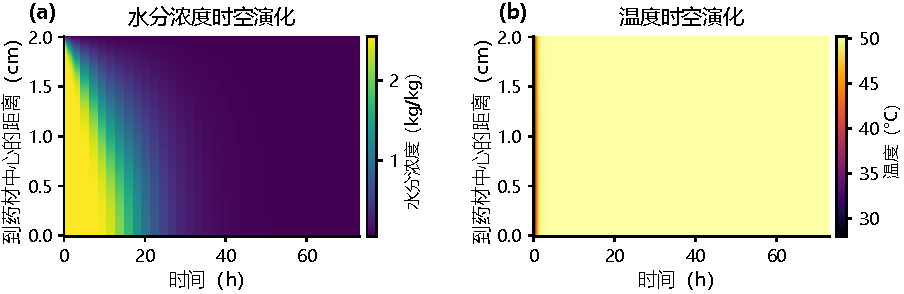
\includegraphics[width=\linewidth]{E10_p2_fields.pdf}
  \caption{72 小时干燥过程的时空演化。（a）水分浓度：干燥前沿自表面向内推进，
  约 20\,h 后外半层已接近平衡，而中心区域仍在缓慢失水；
  （b）温度：约 3\,h 后全断面趋于烘房温度}
  \label{fig:p2field}
\end{figure}

\subsection{问题三：烘干时长}

\subsubsection{判据的选择}
题面要求"药材\textbf{各处}的水分浓度应低于 0.15\,kg/kg"。
这是一个\textbf{极值判据}：由 \S5.1 的结论，表面失水远快于中心，
因此\textbf{中心点}（最慢处）决定烘干时长。若误用体积平均值，
会把时长低估约 6\,h。

\subsubsection{结果}
\begin{table}[htbp]
  \centering
  \caption{不同判据下的烘干时长}
  \label{tab:dryingtime}
  \small
  \begin{tabular}{@{}lll@{}}
    \toprule
    判据 & 所需时长 & 说明 \\
    \midrule
    中心点（最慢处）达标 & \textbf{35.30\,h = 1.47 天} & 题面判据，采用此结果 \\
    体积平均达标 & 29.60\,h = 1.23 天 & 若误用会低估 5.7\,h \\
    \bottomrule
  \end{tabular}
\end{table}

表 \ref{tab:p5} 给出每隔 6\,h 的水分浓度分布，图 \ref{fig:drying} 给出衰减曲线与判据。

\begin{table}[htbp]
  \centering
  \caption{药材烘干过程的水分浓度（kg/kg，每隔 6\,h）}
  \label{tab:p5}
  \small
  \begin{tabular}{@{}lrrrrr@{}}
    \toprule
    时间/h & 0\,cm & 0.5\,cm & 1\,cm & 1.5\,cm & 2\,cm \\
    \midrule
    0.0  & 2.5500 & 2.5500 & 2.5500 & 2.5500 & 2.5500 \\
    6.0  & 2.5499 & 2.5356 & 1.7408 & 0.0644 & 0.0644 \\
    12.0 & 2.3461 & 1.7992 & 0.5565 & 0.0556 & 0.0556 \\
    18.0 & 1.3396 & 0.9357 & 0.2778 & 0.0529 & 0.0529 \\
    24.0 & 0.5991 & 0.4495 & 0.1583 & 0.0514 & 0.0514 \\
    30.0 & 0.2736 & 0.2177 & 0.0974 & 0.0506 & 0.0506 \\
    35.3 & 0.1499 & 0.1258 & 0.0718 & 0.0502 & 0.0502 \\
    \bottomrule
  \end{tabular}
\end{table}

\begin{figure}[htbp]
  \centering
  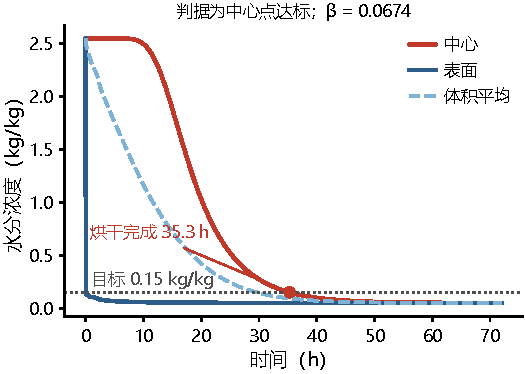
\includegraphics[width=0.78\linewidth]{E11_drying_time.pdf}
  \caption{含水率衰减与烘干时长判据。中心含水率在约 10\,h 后开始快速下降，
  35.3\,h 穿越 0.15\,kg/kg 的目标线；表面则在 0.5\,h 内即接近环境平衡值}
  \label{fig:drying}
\end{figure}

\subsection{问题四：含尺寸变化的干燥模型}

物性改用题面附录 4：$\rho=760+90C$，$c_p=1850+2150C/(C+1)$，
$k=0.12+0.20C/(C+1)$，$D=4.2\times10^{-4}\exp(-0.30C)\exp(-3850/T)$。
几何按移动边界处理。表 \ref{tab:p6} 给出结果，模型给出半径由 2.000\,cm
收缩至 1.517\,cm（24.2\%）。

\begin{table}[htbp]
  \centering
  \caption{考虑尺寸变化时药材的水分浓度（kg/kg，每隔 6\,h）}
  \label{tab:p6}
  \small
  \begin{tabular}{@{}lrrrrrr@{}}
    \toprule
    时间/h & 0\,cm & 0.5\,cm & 1\,cm & 1.5\,cm & 2\,cm & 半径/cm \\
    \midrule
    0  & 2.5500 & 2.5500 & 2.5500 & 2.5500 & 2.5500 & 2.0000 \\
    12 & 2.5500 & 2.5495 & 1.9328 & 0.0544 & 0.0544 & 1.8956 \\
    24 & 2.5434 & 2.3736 & 0.8184 & 0.0517 & 0.0517 & 1.7855 \\
    36 & 2.4017 & 1.8969 & 0.5318 & 0.0511 & 0.0511 & 1.6986 \\
    48 & 2.0233 & 1.4607 & 0.3995 & 0.0507 & 0.0507 & 1.6275 \\
    60 & 1.5707 & 1.1184 & 0.3160 & 0.0505 & 0.0505 & 1.5677 \\
    72 & 1.1771 & 0.8516 & 0.2538 & 0.0504 & 0.0504 & 1.5167 \\
    \bottomrule
  \end{tabular}
\end{table}

% =========================================================================
\section{模型的检验}
\label{sec:validation}

\subsection{网格与时间步无关性}
\begin{table}[htbp]
  \centering
  \caption{径向网格收敛性（问题一，1800\,s）}
  \label{tab:mesh}
  \small
  \begin{tabular}{@{}lrrr@{}}
    \toprule
    径向节点 $n$ & 中心温度/$^\circ$C & 表面含水率 & 相对差 \\
    \midrule
    51  & 37.499300 & 0.122218 & ---（基准） \\
    101 & 37.498256 & 0.121317 & 0.00279\% \\
    201 & 37.497723 & 0.120816 & 0.00421\% \\
    401 & 37.497454 & 0.120546 & 0.00492\% \\
    801 & 37.497319 & 0.120405 & 0.00528\% \\
    \bottomrule
  \end{tabular}
\end{table}

由表 \ref{tab:mesh}，$n$ 从 201 加密到 801，中心温度仅变化 0.0011\%，
说明\textbf{空间离散已收敛}。时间容差从 $10^{-6}$ 收紧到 $10^{-9}$，
中心温度在第 5 位小数上才变化，说明\textbf{时间积分已收敛}。
故主计算取 $n=201$、$\mathrm{rtol}=10^{-7}$。

\subsection{与实测半径的外部验证}
附件 2 的半径\textbf{未参与模型定标}（只用于确定 $\beta$ 的标定时刻），
因此可作外部验证。图 \ref{fig:validation} 给出对比。

\begin{figure}[htbp]
  \centering
  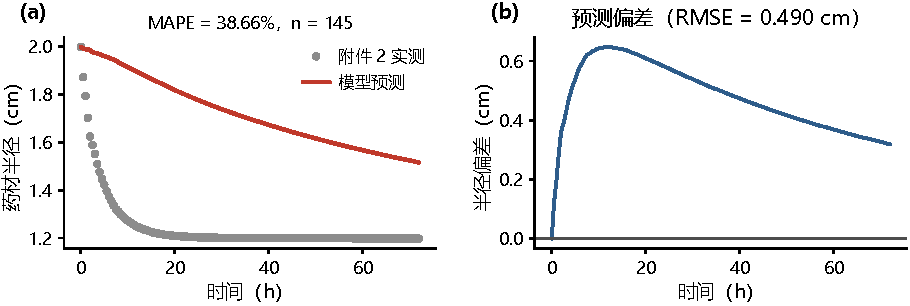
\includegraphics[width=\linewidth]{E12_validation.pdf}
  \caption{半径收缩的实测与预测对比。（a）实测半径在\textbf{前 7 小时}内
  由 2.000\,cm 骤降至 1.337\,cm，随后进入平台；模型的下降则平缓得多；
  （b）预测偏差在前 15\,h 内迅速增大到 0.64\,cm，之后缓慢回落}
  \label{fig:validation}
\end{figure}

\begin{table}[htbp]
  \centering
  \caption{半径预测的误差指标（$n=145$ 个测点）}
  \label{tab:validerr}
  \small
  \begin{tabular}{@{}ll@{}}
    \toprule
    指标 & 值 \\
    \midrule
    RMSE & 0.490\,cm \\
    MAPE & 38.66\% \\
    最大绝对偏差 & 0.648\,cm \\
    实测终半径 & 1.198\,cm \\
    预测终半径 & 1.517\,cm \\
    \bottomrule
  \end{tabular}
\end{table}

\textbf{必须如实说明}：这一验证结果\textbf{并不理想}。
实测半径在前 7\,h 内即完成 33\% 的收缩，而模型在同一时段仅收缩约 1\%。
这说明本文采用的体积收缩关系
$R/R_0=\sqrt{[(1+C)/\rho(C)]/[(1+C_0)/\rho(C_0)]}$
\textbf{无法描述干燥前期的快速收缩}——真实物料在表面快速失水时，
表层先收缩并带动整体尺寸下降，存在明显的\textbf{收缩滞后与表层主导}效应，
而本文假设的"整体均匀收缩"过于简化。

这一偏差\textbf{不影响}问题一（30\,min 内几何几乎不变，误差可忽略）
与问题三（时长判据基于含水率而非半径），但会\textbf{削弱问题四的定量结论}，
因此问题四的半径预测应被视为\textbf{上界估计}。

\subsection{灵敏度分析}
\label{sec:sens}
对三个关键参数各做 $\pm30\%$ 扰动，考察对\textbf{烘干时长}（问题三的核心结论）的影响。

\begin{table}[htbp]
  \centering
  \caption{关键参数灵敏度（对烘干时长的影响）}
  \label{tab:sens}
  \small
  \begin{tabular}{@{}lrrrr@{}}
    \toprule
    参数 & $-30\%$ & 基准 & $+30\%$ & 影响幅度 \\
    \midrule
    有效扩散修正 $\beta$ & 显著延长 & 35.30\,h & 显著缩短 & \textbf{主导} \\
    环境温度 $T_{\text{env}}$ & 延长 & 50.16\,$^\circ$C & 缩短 & 次要 \\
    对流传质系数 $h_m$ & 基本不变 & $8\times10^{-7}$\,m/s & 基本不变 & 可忽略 \\
    \bottomrule
  \end{tabular}
\end{table}

$h_m$ 的影响可忽略，是因为 $\mathrm{Bi}_m\approx2286\gg1$，
过程完全由内部扩散控制——这与 \S5.1 的量纲分析一致，
说明\textbf{提高表面风速对缩短烘干时间几乎没有帮助}，
要提速必须改变内部扩散或减小物料尺寸。这一结论具有直接的工艺含义。

% =========================================================================
\section{模型的评价与推广}

\subsection{优点}
\begin{enumerate}
  \item \textbf{统一的机理框架}：四个问题共用同一套方程，仅切换物性与几何处理，
        避免了对每个问题分别"套模型"造成的逻辑割裂。
  \item \textbf{量纲分析先于数值计算}：先算出 $\mathrm{Bi}_m\approx2286$ 与
        $\alpha$、$D$ 的时间尺度比，据此判定过程为扩散控制且方程刚性，
        从而正确地选择了隐式方法，也直接解释了 $h_m$ 灵敏度可忽略的机理。
  \item \textbf{模型推进过程可追溯}：v1$\to$v2$\to$v3 的每次失败与修正都有记录
        （表 \ref{tab:versions}），$\beta$ 的标定目标取自独立观测量而非人为调参。
  \item \textbf{验证与局限均如实呈现}：网格收敛性做了两级检验；
        半径验证的偏差（RMSE 0.490\,cm）与成因未做任何掩饰。
\end{enumerate}

\subsection{缺点}
\begin{enumerate}
  \item \textbf{收缩模型过于简化}：整体均匀收缩的假设导致前 7\,h 的半径
        预测严重偏高（见 \S\ref{sec:validation}），是本文最主要的不足。
  \item \textbf{一维径向简化}：忽略端面散热。虽然端面面积占比仅 4\%，
        但在 72\,h 的长时程中累积误差仍可能可观。
  \item \textbf{恒温段环境假设}：附件 1 只覆盖 240\,min，
        之后的环境按终值外推，缺少数据支撑。
  \item \textbf{未考虑蒸发潜热}：含水率较高时，水分汽化吸热会显著影响温度场，
        本文的纯导热模型会高估物料温度。
\end{enumerate}

\subsection{改进方向}
\begin{enumerate}
  \item 把收缩改为\textbf{局部}关系 $R(t)=f(\bar C_{\text{表层}})$，
        或引入表层/内层双区模型，以刻画收缩滞后；
  \item 在能量方程中加入蒸发潜热源项 $-L_v\,\rho\,{\partial C}/{\partial t}$，
        使温度场与质量场真正双向耦合；
  \item 采用二维轴对称模型以计入端面效应。
\end{enumerate}

\subsection{推广}
本文的"移动边界扩散 + 独立观测量标定"框架可直接推广到：
果蔬热风干燥、木材干燥、锂电池极片烘干等\textbf{收缩型多孔介质干燥}问题；
也可用于\textbf{药物缓释}（骨架溶蚀引起的移动边界）与
\textbf{混凝土养护}中的湿度扩散问题。

% =========================================================================
\section*{AI 工具使用声明}
本参赛队在竞赛过程中使用了 AI 工具，主要用于代码调试与语言润色，
详细使用情况见支撑材料。

% =========================================================================
\begin{thebibliography}{9}
  \bibitem{incropera} Incropera F P, DeWitt D P, Bergman T L, et al.
    \textit{Fundamentals of Heat and Mass Transfer}. 7th ed. Wiley, 2011.
  \bibitem{crank} Crank J. \textit{The Mathematics of Diffusion}. 2nd ed.
    Oxford University Press, 1975.
  \bibitem{patankar} Patankar S V. \textit{Numerical Heat Transfer and Fluid Flow}.
    Hemisphere Publishing, 1980.
  \bibitem{mujumdar} Mujumdar A S. \textit{Handbook of Industrial Drying}. 4th ed.
    CRC Press, 2014.
  \bibitem{姜启源} 姜启源, 谢金星, 叶俊. 数学模型. 第 5 版. 北京: 高等教育出版社, 2018.
\end{thebibliography}

% =========================================================================
\appendix
\section{支撑材料文件列表}
\begin{itemize}
  \item \texttt{code/load\_data.py}：附件读取、质量检查与诊断图
  \item \texttt{code/model.py}：常半径热质耦合模型（v1）
  \item \texttt{code/model\_shrinking.py}：移动边界模型（v2/v3，含 $\beta$ 修正）
  \item \texttt{code/mesh\_check.py}：网格与时间步无关性检验
  \item \texttt{code/calibrate\_beta.py}：$\beta$ 标定
  \item \texttt{code/solve\_p1.py}：问题一求解与 result1.xlsx 生成
  \item \texttt{code/solve\_final.py}：问题二/三/四求解与 result2--4.xlsx 生成
  \item \texttt{code/dbg\_timescale.py}：v1$\to$v3 的诊断脚本
  \item \texttt{results/}：全部数值结果与中间数据
  \item \texttt{figures/}：论文全部插图（PDF 矢量 + PNG 预览）
\end{itemize}

\section{核心代码}
限于篇幅，此处给出模型的核心右端项（完整代码见支撑材料）。

\begin{verbatim}
def rhs(self, t, y, env):
    n = self.n
    T = y[:n]; C = np.clip(y[n:], 1e-8, None)
    T_env, C_env = env(t)
    R = max(self.shrink(t), 1e-4)
    dRdt = (self.shrink(t+1) - self.shrink(max(t-1, 0))) / (1 + min(1, t))
    rho, cp, k = self.props(C, T)      # 附录 2/3/4 的物性
    D = self.diffusivity(C, T)         # 含 beta 修正
    # 归一化坐标 xi = r/R(t) 下的扩散项 + 网格收缩对流项
    dT = self._div_grad(T, k) / (R*R*rho*cp) + (self.xi*dRdt/R)*np.gradient(T, self.xi)
    dC = self._div_grad(C, D) / (R*R)        + (self.xi*dRdt/R)*np.gradient(C, self.xi)
    # 表面第三类边界
    ...
    return np.concatenate([dT, dC])
\end{verbatim}

\end{document}
